\input{common_packages.tex}

\begin{document}

\title{\textbf{Parameter Manager} \\
\large\textit{Component Design Document}}
\date{}
\maketitle

\section{Description}
\input{build/tex/parameter_manager_description.tex}

\section{Requirements}
\input{build/tex/parameter_manager_requirements.tex}

\section{Design}

\subsection{At a Glance}
\input{build/tex/parameter_manager_stats.tex}

\subsection{Diagram}
\begin{figure}[H]
  \includegraphics[width=1.0\textwidth,center]{../build/eps/parameter_manager.eps}
  \caption{Parameter Manager component diagram.}
\end{figure}

\subsection{Connectors}
\input{build/tex/parameter_manager_connectors.tex}

\subsection{Initialization}
\input{build/tex/parameter_manager_init.tex}

\subsection{Commands}

\input{build/tex/parameter_manager_commands.tex}

\subsection{Events}

\input{build/tex/parameter_manager_events.tex}

\subsection{Packets}

\input{build/tex/parameter_manager_packets.tex}

\section{Unit Tests}

\input{build/tex/parameter_manager_unit_test.tex}

\section{Appendix}
\subsection{Packed Types}

\input{build/tex/parameter_manager_types.tex}

\subsection{Enumerations}

\input{build/tex/parameter_manager_enums.tex}

\end{document}
